%!TEX root = ../thesis-guntur.tex
%************************************************
\chapter{Experimental Setup}
\label{ch:experimental-setup} % $\mathbb{ZNR}$
%************************************************
% \marginpar{Use this to write down some comments.}

In this chapter, we present our proposed experiment, along with the goals and how to set it up. We plan to devise a social density estimation, which could replace the manual counting method. We aim to implement this estimation as a passive behavioral monitoring system in which smartphones are used as measuring instruments. The estimation may allow us to differentiate between healthy and non-healthy individuals, especially related to neuropsychiatric disorders.

We start with general experimental design of smartphone based social density estimation. We then explain the technical implementation of our initial experiment design. Lastly, we present the method of data extraction from collection of raw log files and how we evaluate the data.








\section{Experimental Design} % (fold)
\label{sec:experimental_design}
% - context: what is the experiment about, what is the goal of the experiment, how can one set it up. No reference to hardware, OS, software should be here.
In the present study, we would like to know whether we can use smartphone sensor readings as a way to estimate the level of social density in the surroundings. To do so, we compare the level of social density with the smartphone sensor readings, collected from subjects under real world condition. We try to get wide range of social density levels, from low to high social density level, and we try to employ as many sensors as possible.

% how to count people: manually, semi-electronic (photos), fully electronic
It is known that getting the ground truth of the actual social density level in public spaces is difficult~\cite{thesis041}. As an option, we use estimation approach. There are several means to estimate social density level, for instance, manual counting of people using tally counter as what retail stores do, manual counting by taking notes on paper, manual head counting on captured pictures, and electronic based counting. In the present study, we employ manual and electronic-based method, by using head count of captured pictures and unique device counting. We select two methods so that we can get more insight of the actual social density condition.

% what smartphone sensors to use
Modern smartphones are equipped with broad range of sensors, such as
\begin{enumerate*}[label={\alph*)},font={\color{red!50!black}\bfseries}]
  \item Bluetooth,
  \item WiFi,
  \item microphone,
  \item NFC,
  \item camera,
  \item cellular network card,
  \item touch screen,
  \item fingerprint,
  \item accelerometer,
  \item gyroscope,
  \item proximity,
  \item compass, and
  \item barometer.
\end{enumerate*}
However, not all of them are exploitable for estimating the level of social density. We have selected several sensors which are potentially usable especially for passive monitoring. We select WiFi and microphone to estimate the social density level because those sensors are able to perceive the surroundings no matter how the smartphone is operated and positioned.

% location and timing
To collect samples of real world condition with high variation of social density level, we selected locations that represent low and high social densities as well as indoor and outdoor locations. We plan to do our experiment where WiFi \ac{AP} use is not restricted, i.e., people are free to set up their own WiFi \ac{AP} in anyway they prefer. Some locations where the use of WiFi is restricted exist, for instance, University of Groningen complex. In the university complex, \verb|eduroam| is the only the official available \ac{AP} and the occupants are discouraged to install their own \ac{AP}. Thus, making this not suitable for our study.

% investigate the effect of time
We collect the data of a certain location once per day, when the location gets its maximum number of visitor. To get the insight of the variation between days, we collect the data in several days of experiment. Furthermore, as social density level in a certain location is very dynamic, we also conduct several data collections per day, e.g., taken at 09:00, 12:00, and so on, at a single location.

% what is the result and what we are trying to evaluate
In the present study, we evaluate the correlation of social density level and the smartphone sensor readings. If the social density level and smartphone sensor readings have a correlation, we can say that it is possible to estimate the level of social density using smartphone sensor readings but we have to further investigate the accuracy and the limitation of this approach. We also examine the variation of the correlation in different scanning days and scanning time.











\section{Implementation} % (fold)
\label{sec:implementation}
% start with general remarks
In this section, we describe how we implement our proposed experimental design mentioned before. We firstly study the behavior of \ac{MAC} address randomization, observed in both Android and iOS devices~\cite{thesis061}, to minimize the bias in device count based social density level estimation. Then, we describe the method we use to estimate the social density level. We also specify the smartphone sensors that we use in the present study and their corresponding outcomes, followed by a description of the different location and timing setup. Lastly, we finalize with an explanation about technical scanning mechanism.

% randomization
\subsection{MAC Address Randomization Investigation} % (fold)
\label{sub:mac_address_randomization_investigation}
\ac{MAC} address randomization allows WiFi enabled devices to rearrange or change their \ac{MAC} address in particular circumstance to increase the privacy of the user. The randomized \ac{MAC} address uses locally administered address, which is indicated by the second-least-significant bit of the first octet of the address~\cite{thesis082}. The original \ac{MAC} address uses universally administered address, which is uniquely assigned by its manufacturer.

We capture the probe request packets from nearby WiFi-enabled devices and store the captured information to a log file. Probe request is a data packet broadcast by WiFi-enabled devices to scan for available \ac{AP}. This mechanism is part of active scanning in WiFi standards~\cite{thesis082}, which is more energy efficient than passive scanning.

In the current investigation, we note 
\begin{enumerate*}[label={\alph*)},font={\color{red!50!black}\bfseries}]
  \item the timing when the randomized MAC address appears,
  \item the \ac{SN} field\footnote{The \ac{SN} field is a 12-bit field indicating the sequence number of a probe request packet. This marks the order of how the packets are broadcasted.} of the packet, and
  \item the variation of the \ac{MAC} address.
\end{enumerate*}

We investigate the randomization behavior in both iOS, using iPad mini with iOS 10.0, and Android, with LG Nexus 5X with Android 6.0 (Marshmallow). When experimenting on iPad mini, we turn the LG Nexus 5X off, and vice versa, to make sure that each device is not disturbing each other. We do this experiment within 30 minutes for each device.

We choose a remote area where we cannot detect any other probe request except from our device to perform the experiment. We use Wireshark\footnote{\url{https://www.wireshark.org}}, a popular network protocol analyzer software, to capture and store the captured probe request packets to a \verb|pcap| file. We run this experiment on Apple's MacBook Air with built-in WiFi card that supports monitor mode.

% people counting
\subsection{Social Density Estimation} % (fold)
\label{sub:social_density_estimation}
We use two approaches to estimate the crowd count in the surroundings, by using manual counting on photographic images and unique \ac{MAC} address counting from captured probe request. We estimate the crowd count as a first approximation of the ground truth because it is known that getting the ground truth of crowd density in public spaces is difficult~\cite{thesis041}.

	\subsubsection{Device Count Based Estimation} % (fold)
	\label{ssub:probe_request_based_estimation}
	We count unique device in the surroundings by capturing probe request packets broadcast by nearby devices and taking note on the unique \ac{MAC} addresses. Counting the unique \ac{MAC} address will result in a list of unique device in the surroundings. We decide to implement unique \ac{MAC} address counting in probe request as it is proven to be a promising method to estimate crowd count~\cite{thesis047}.

	In device count based estimation, we capture the probe request packets in WiFi channel 1 (2.4 GHz). We are not capturing packets in other WiFi channels as WiFi-enabled device will broadcast the probe requests to all available WiFi channels~\cite{thesis082}. Furthermore, capturing packets in every WiFi channels is not doable on a single device, due to the limitation of a device of being only in a certain WiFi channel at a time. Capturing packets in multiple channels requires channel hopping, i.e., hopping from one channel to another within a short time interval, which is considered a lossy method and prone to losing some probe request packets.
	

	\subsubsection{Manual Head Counting in Photographic Images} % (fold)
	\label{ssub:manual_counting_using_photo}
	In addition to device count based estimation, we incorporate another crowd counting estimation method using photographic images. We consider this method as an estimation of the ground truth, as photographic images are subject to light and sight, i.e., physical obstacle would interfere the final result.
	
	% comparison of image based counting
	We prefer photographic images that support wide \ac{FOV}, i.e., able to cover 360 degrees of horizontal \ac{FOV}. Some of the options that we consider are panoramic photograph and wide-angle photograph. During our early testing, panoramic photograph using smartphone suffers from misaligned images, as panoramic photograph is a computer-based concatenated images taken in different timestamp. This causes some object to appear more than once, or even not at all. Thus, we decide to use wide-angle photograph to achieve 360 degrees of horizontal \ac{FOV}.

	\begin{figure}[ht]
	\centering
	\subfloat[illustration]{\label{fig:gopro-mdleft}{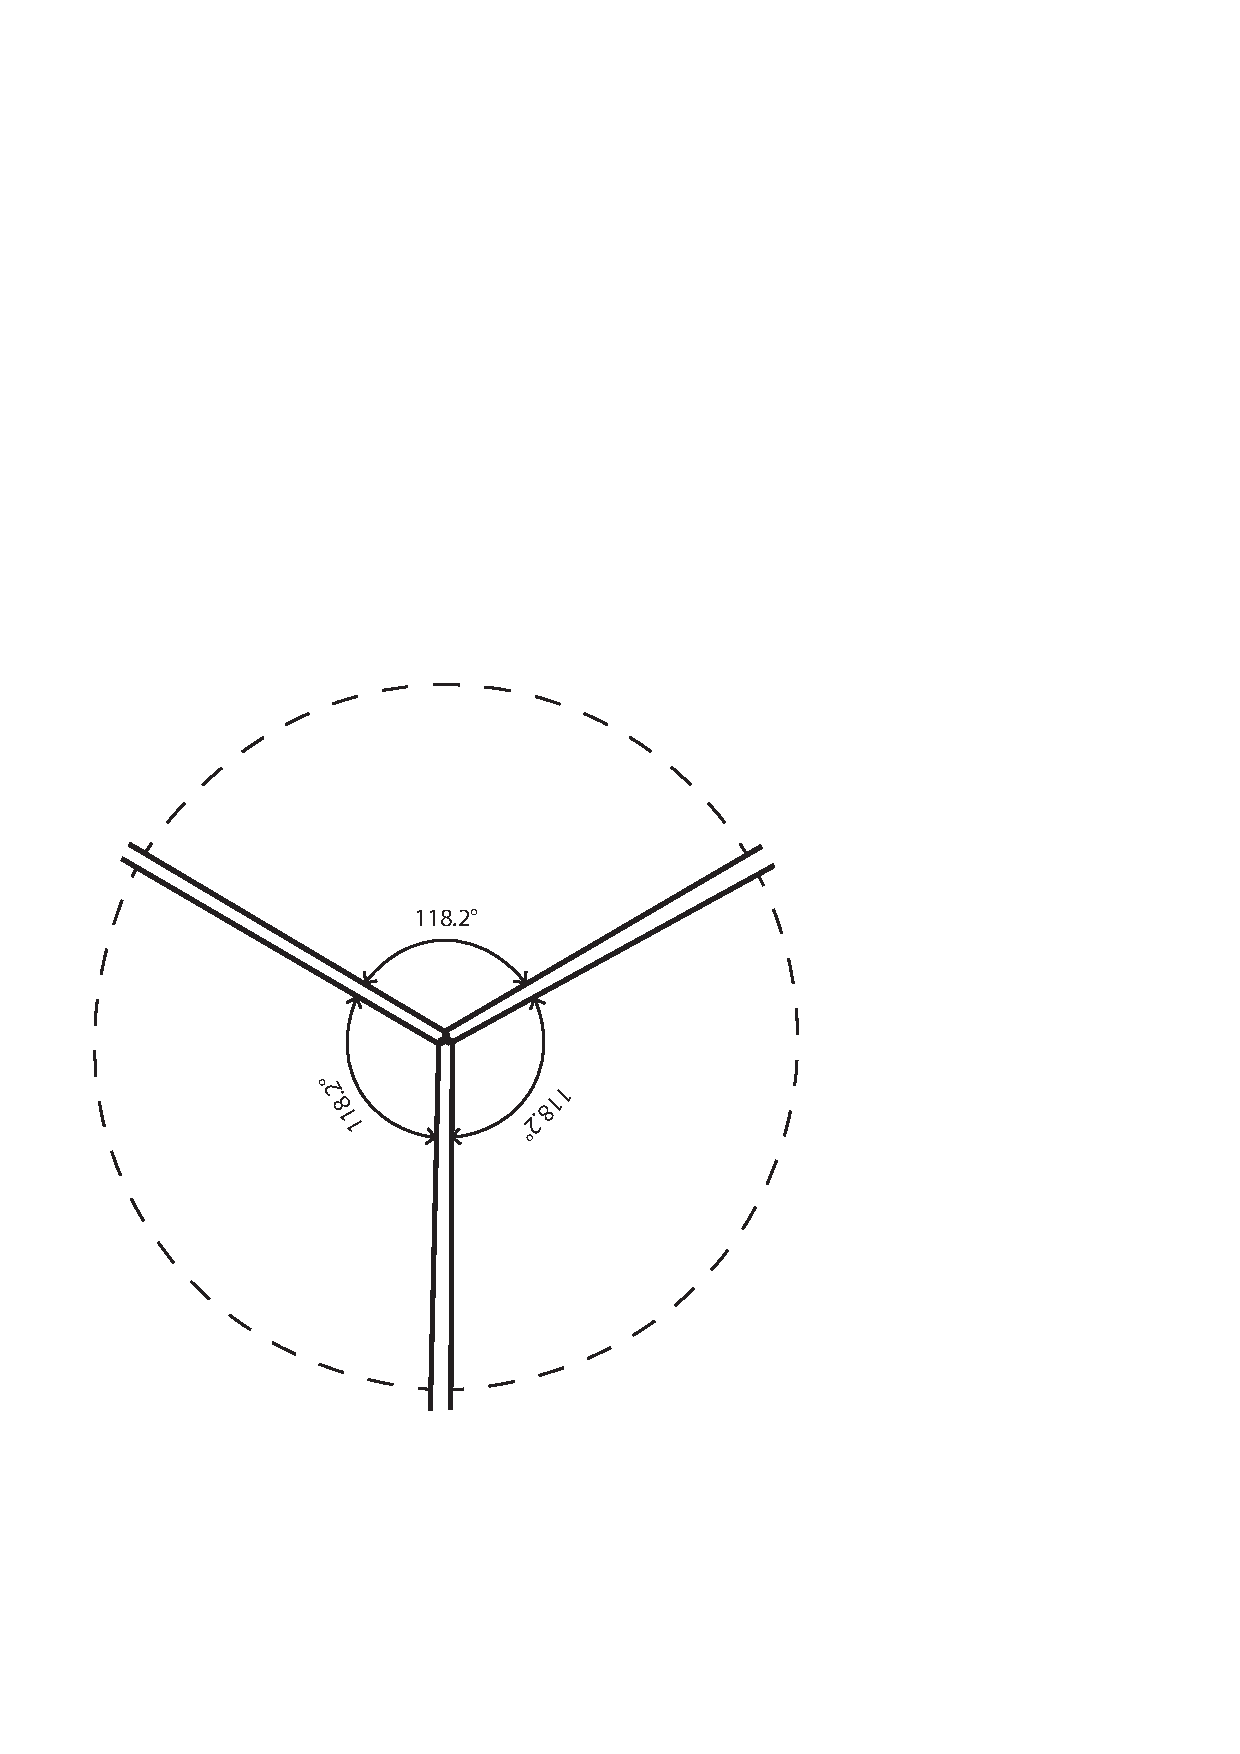
\includegraphics[width=0.4\textwidth]{./img/3-gopro-setup}}}\hfill
	\subfloat[implementation]{\label{fig:gopro-mdright}{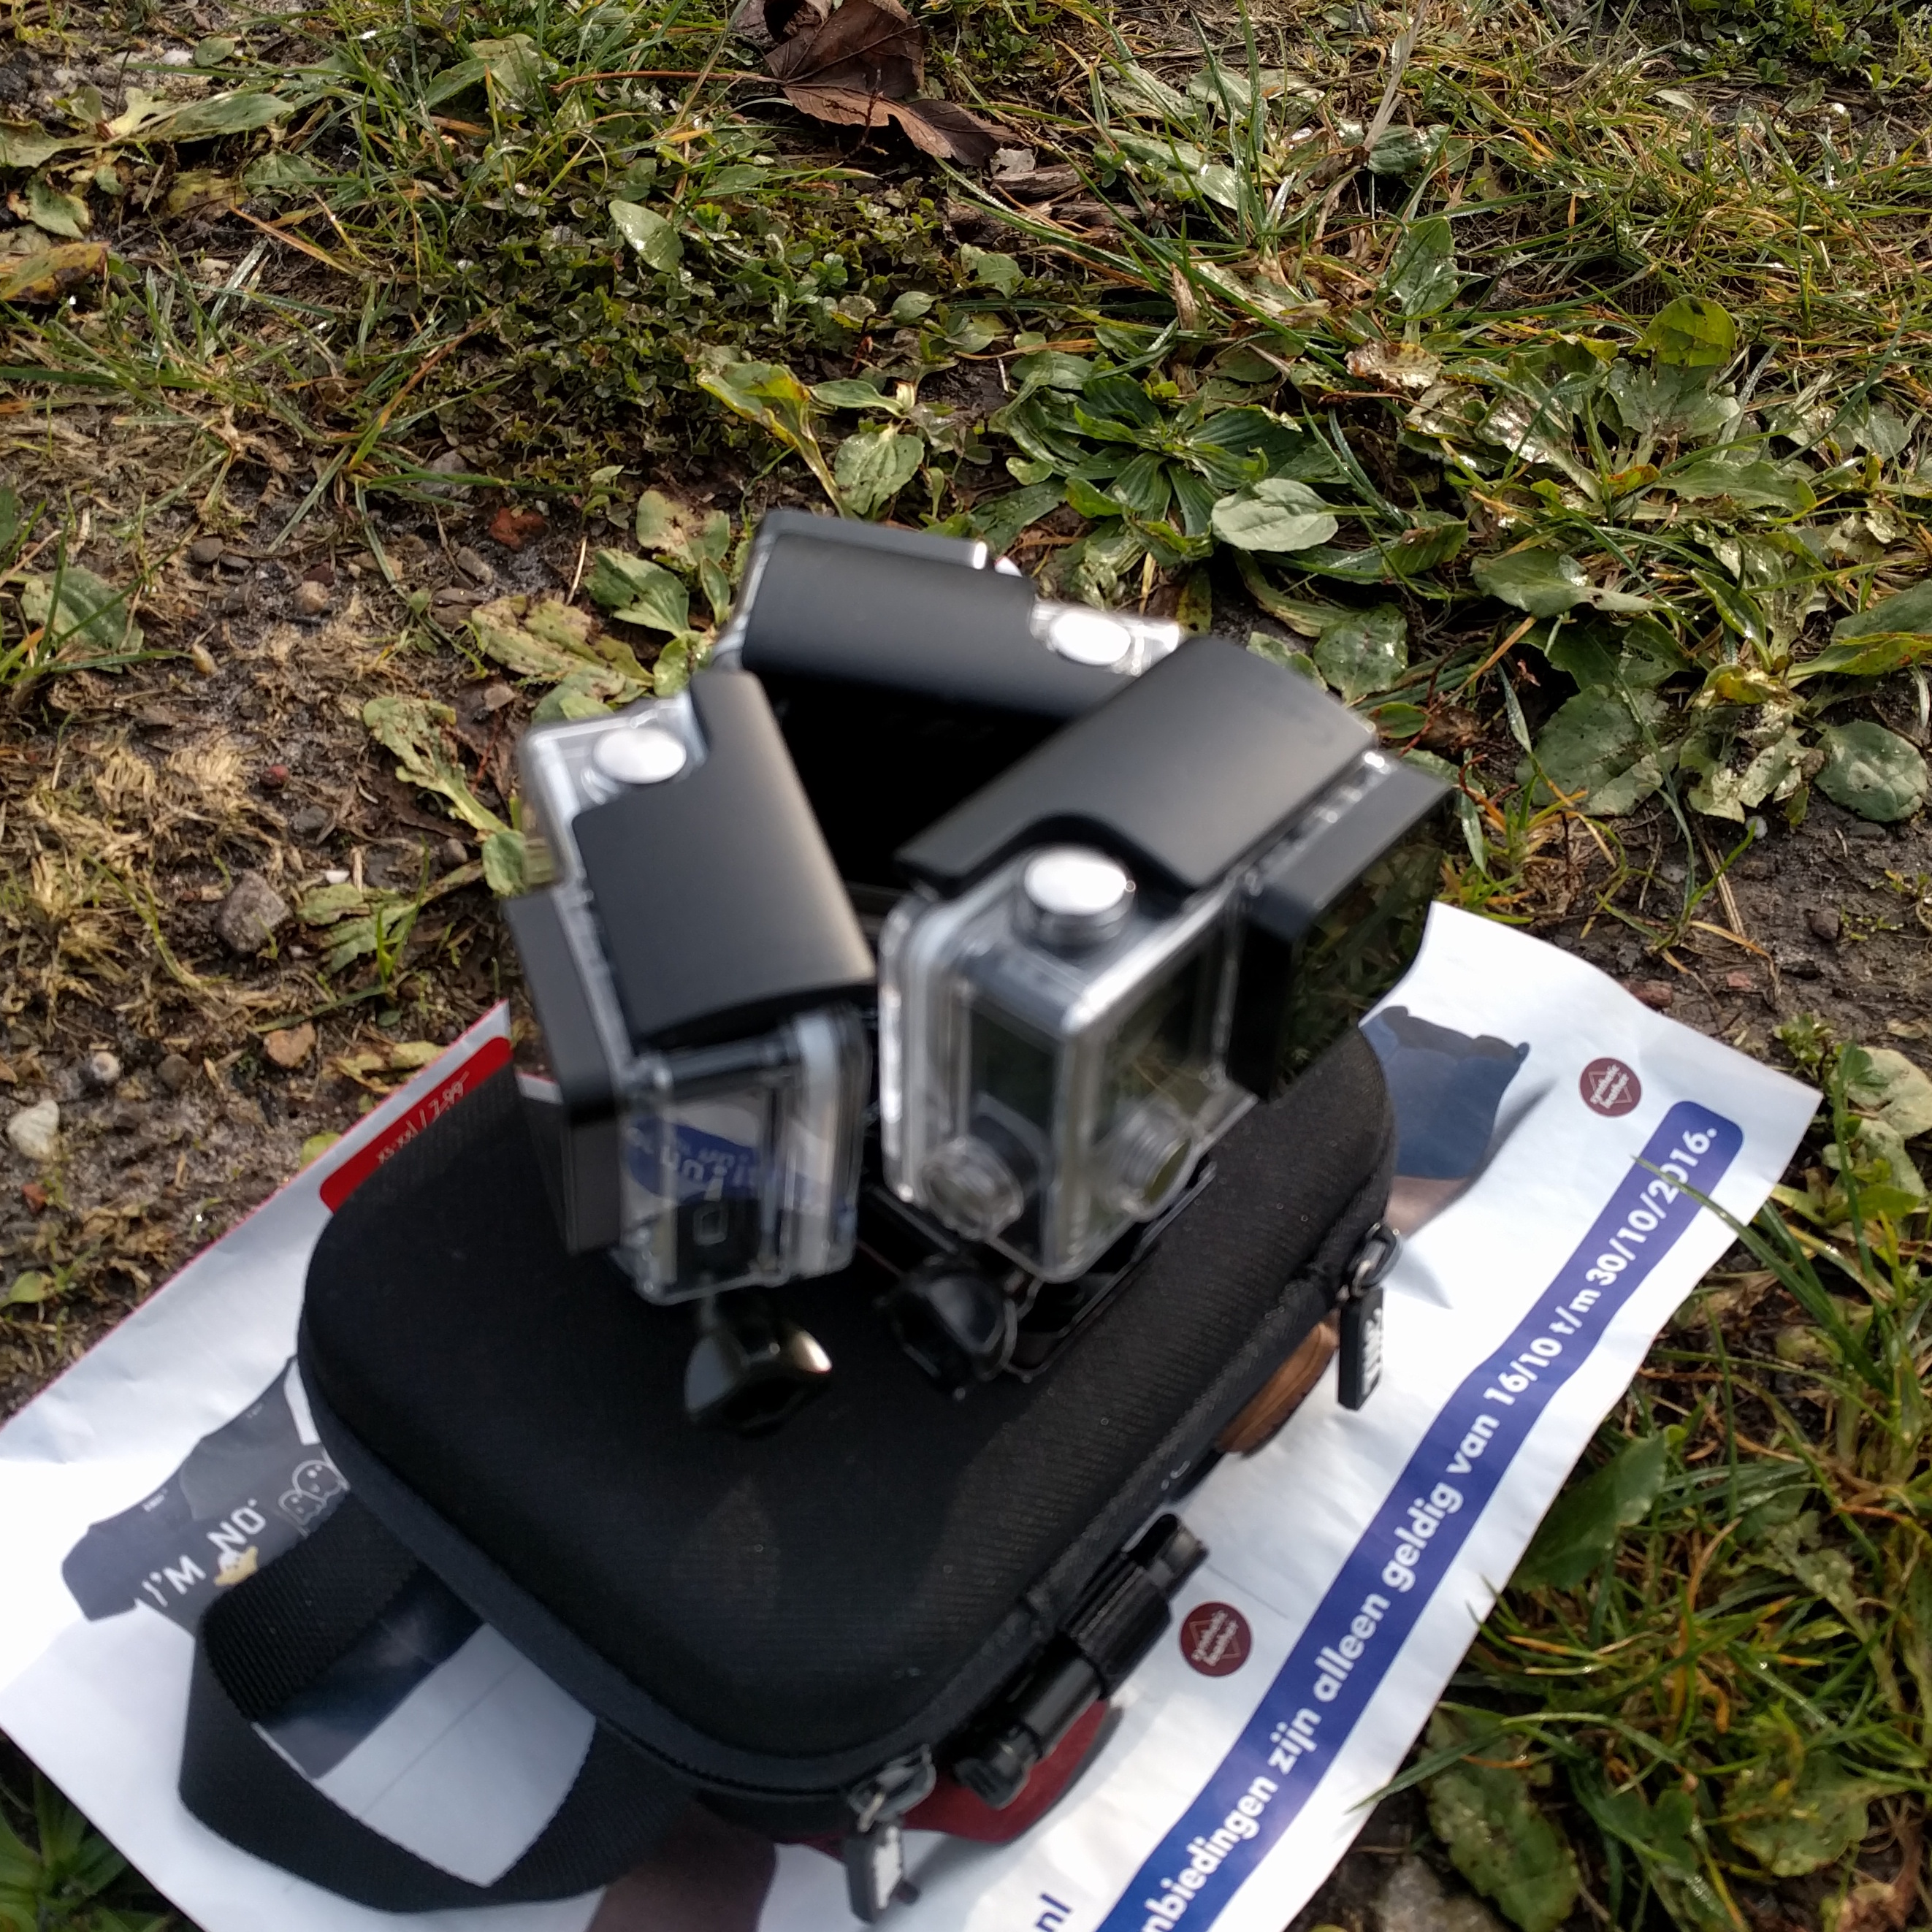
\includegraphics[width=0.4\textwidth]{./img/3-gopro-setup-pict}}}
	\caption[GoPro arrangement]{GoPro arrangement to achieve 360 degrees of horizontal \ac{FOV}.}
	\label{fig:gopro-placement}
	\end{figure}

	% setup, picture or vide, why?
	We use GoPro\footnote{\url{https://gopro.com}} Hero4 silver wide-angle action camera to get the photographic image. According to GoPro technical specifications~\cite{goprofieldofview}, its maximum horizontal \ac{FOV} is 118.2 degrees in 16$x$9 wide mode with 17.2mm focal length. To achieve 360 degrees of \ac{FOV}, we use three GoPro cameras positioned in circular arrangement, as depicted in ~\autoref{fig:gopro-placement}. Although some blind spots are still present, this setup is still able to capture objects within intended range.

	% we use timelapse, why: battery and memory limit
	We employ time-lapse photography technique to capture the surroundings in preference to normal video capture. We capture a still image each five seconds, resulting 12 still images per minute. We do not employ video recording to conserve GoPro battery. As stated in GoPro technical specification of battery life~\cite{goprobattery}, estimated battery life of taking video is roughly two hours, while our experiment is planned to be more than two hours (plus back-up time). We consider changing battery during data collection is impractical. Moreover, taking time-lapse images would increasingly save more data storage.
	
	In the end, we manually do head counting based on captured images grouped in each time interval. We make sure that one person is counted once to avoid counting the same person multiple times.

% smartphone sensor reading
\subsection{Smartphone Sensor Utilization} % (fold)
\label{sub:smartphone_sensor_utilization}
We use WiFi and microphone as sensors because those sensors are able to perceive the surroundings no matter how the smartphone is operated and positioned. This means that the passive monitoring process can still running in background regardless how user use the smartphone. In the other hand, camera based approach requires the smartphone to be positioned accordingly to be able to capture appropriate images for crowd counting.

	\subsubsection{WiFi scanning} % (fold)
	\label{ssub:wifi_scanning}
	Ideally, we use probe request based crowd estimation, as discussed in~\autoref{ssub:probe_request_based_estimation}, directly in the smartphone. However, this is not possible due to restrictions of the mobile operating system. Probe request based estimation only works in WiFi monitor mode~\cite{thesis052,thesis079} and monitor mode is only accessible if the smartphone is rooted, jailbroken, or installed in custom \ac{ROM}, which is considered as illegal in most countries~\cite{rootjailbreak}.
	
	We count the available \ac{AP} nearby and observe its signal strength in place of unique \ac{MAC} address counting in probe request packets. We take note of \ac{AP}'s \ac{BSSID}, which is unique and based on \ac{MAC} address. We are not particularly interested in \ac{AP}'s \ac{SSID} because there might be multiple \ac{AP}s with the same \ac{SSID}. We measure the signal strength of the \ac{AP} in \ac{RSSI}.

	\subsubsection{Ambient Noise Recording} % (fold)
	\label{ssub:ambient_noise_recording}
	In addition to WiFi scanning, we also record the ambient noise to perceive nearby condition, assuming that more crowded locations will have high ambient noise, while less crowded locations will have low ambient noise. We measure the ambient noise in decibels (dB). Moreover, we implement speaker count algorithm based on unsupervised learning method proposed by Xu et al~\cite{thesis067}. This approach will estimate how many persons are speaking in the audio recording.

% location
\subsection{Location and Timing} % (fold)
\label{sub:location_and_timing}
We select four different locations that represent low and high crowd densities as well as indoor and outdoor locations. \autoref{tab:location-summary} summarizes our location selection.

To save GoPro battery, we select 30 minutes as the scanning duration in each location. As we are picking four different locations, this would sum up to two hours of image capture. We also select daytime as the preferred scanning time because that is the time when most crowd are observable.

\begin{table}[]
\centering
\caption[Summary of location selection]
{Summary of location selection for the experiment. We plan to run the experiment from Wednesday to Saturday, October 26\textsuperscript{th} to 29\textsuperscript{th}, 2016.}
\label{tab:location-summary}
\begin{tabular}{llll} \toprule
Location                  & Type    & Crowd Level & Scanning Time \\ \midrule
Remote area               & outdoor & low         & 11:00-11:30   \\
Home                      & indoor  & low--medium  & 08:15-08:45   \\
Paddepoel shopping center & indoor  & medium--high & 14:45-15:15   \\
Grote markt               & outdoor & high        & 12:00-12:30  \\ \bottomrule
\end{tabular}
\end{table}

% where is it, the maximum visitor [cite] where the scanner sit, is it indoor or outdoor.

% remote
Speaking of the location selection, remote area is a far-off outdoor location located in Paddepoelsterweg, Groningen. The surroundings are mostly trees and grasses. No visible buildings or dwellings exist but there is only a narrow asphalt pathway where sometimes people or vehicles pass by. Approximately no more than 5 individuals are present at the same time. We carry out the experiment in this area during daytime, from 11:00 to 11:30.

% home
Aside from the remote area where the crowd is less likely to be observed, we conduct a data collection at home during breakfast time, from 08:15 to 08:45. This indoor location is located at Planetenlaan 264, Groningen. Currently, there are only 6 inhabitants living in the house. However, people sometimes pass by in front of the house and they might influence the measurement result.

% paddepoel
Padeppoel shopping center is an indoor shopping center located in Paddepoel district, Groningen. The shopping center, which is 14.920 m\textsuperscript{2} in size, holds around 90 shops~\cite{paddepoelstat}. According to statistics~\cite{paddepoelstat}, it has approximately 90.000 visitors per week. We perform the experiment during the peak hours, which is from 14:45 to 15:15.

% grote markt
Grote markt is a open city square which is located in the center of Groningen city. This location is able to hold roughly 8000 visitors at the same time, according to the official government statement~\cite{GemeenteGroningen2016}. We are planning to do data collection in Grote Markt around mid day, from 12:00 to 12:30.

To see the variance between days, we plan to do the experiment in four days, ranging from weekdays to weekend. We plan to run the experiment from Wednesday to Saturday, October 26\textsuperscript{th} to 29\textsuperscript{th}, 2016. We stick to the same schedule for each location.

\subsubsection{Effect of Scanning Time} % (fold)
\label{ssub:effect_of_scanning_time}
We also conduct an experiment aiming at seeing the variance between scanning times. We select Grote Markt in Groningen as the scanning location because Grote Markt is the location in which the level of social density is the highest among the other three locations that we choose (\autoref{sub:location_and_timing}). The four different scanning time are
\begin{enumerate*}[label={\alph*)},font={\color{red!50!black}\bfseries}]
  \item 09:00,
  \item 12:00,
  \item 15:00,
  \item and 18:00
\end{enumerate*},
taken in the same day. The rest of the experimental setup of this process remains the same as previous experiment. However, we do not employ GoPro time-lapse image capture.

% scanning mechanism
\subsection{Scanning Mechanism} % (fold)
\label{sub:scanning}
In summary, we use three inputs to collect and to perceive the surroundings, namely WiFi, microphone, and wide-angle camera. The data collection process is split into several small cycles of $x$ minutes to avoid biased result caused by randomized \ac{MAC} address. The $x$ will be determined by the \ac{MAC} address randomization experiment described in~\autoref{sec:mac-address-randomization}. We keep repeating the cycle until we reach 30 minutes. \autoref{fig:sensor-measurement} depicts the description of each cycle.

\begin{figure}[ht]
	\centering
	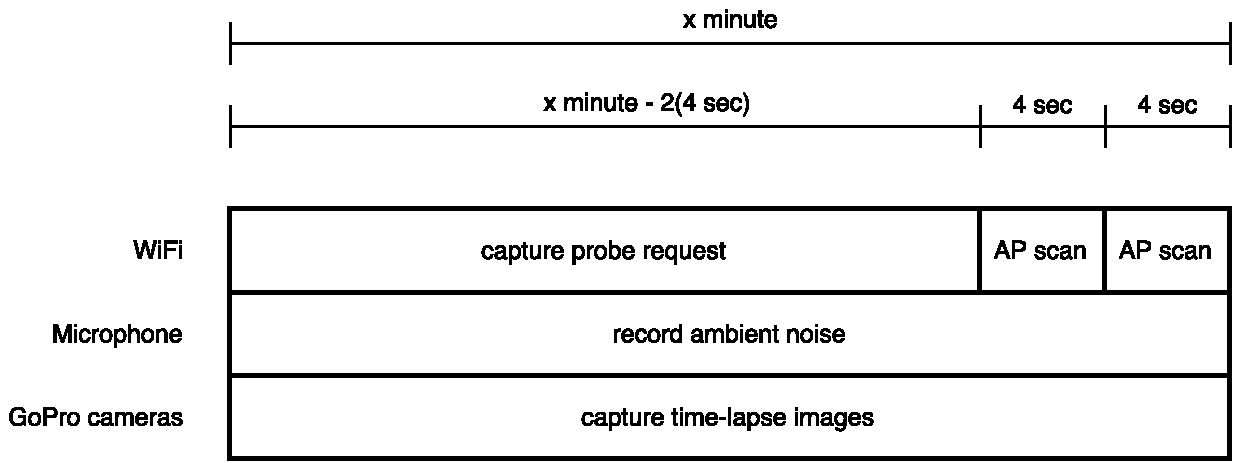
\includegraphics[width=\textwidth]{./img/3-scanning-mechanism}
	\caption{Sensor measurement in each cycle.}
	\label{fig:sensor-measurement}
\end{figure}

% design
As depicted in~\autoref{fig:sensor-measurement}, we work with WiFi to capture the probe request and count the number of available \ac{AP}. We cannot perform these tasks simultaneously, because capturing probe request must be carried out in the WiFi monitor mode. Monitor mode is one of the seven modes, namely master (acting as an \ac{AP}), managed (acting as a WiFi client), ad-hoc, mesh, repeater, and promiscuous, that 802.11 WiFi cards can operate in~\cite{thesis082}. Being in monitor mode, the WiFi card is disconnected from any wireless networks. Thus, we decide to firstly capture probe request before counting the available \ac{AP}. We count the available \ac{AP} twice to achieve better stability. Both microphone and GoPro cameras continuously recording ambient noise and capturing time-lapse images in each cycle.

% technical, both hardware and software
We use Apple MacBook Air, with built-in WiFi card and microphone, as a WiFi scanning and audio recording device. To capture probe request, we use \verb|tcpdump|\footnote{\url{http://www.tcpdump.org}}, a free packet analyzer that runs under the command line, and we use console based Apple's AirPort utility, a software designed by Apple to manage WiFi network, to count available access point. The output of probe request capture is \verb|.pcap| file, a standard file for capturing network traffic. \ac{AP} counting results in plain text files. We work with console based audio editing software, Sound Exchange\footnote{\url{http://sox.sourceforge.net}}, to record the ambient noise to \verb|.wav| file format.

To automate the WiFi scanning and audio recording process, we write a bash script\footnote{Bash script is a list of Bash commands that run on console based application to execute particular tasks.}. We label the resulting log files in the corresponding timestamp and location. Our code is publicly available online\footnote{\url{https://github.com/gtrdp/masters-thesis-guntur}}.













\section{Data Extraction and Evaluation} % (fold)
\label{sec:data_extraction_and_evaluation}
In each cycle of data collection, we obtain approximately 1,170 raw files in many different formats. The files are, namely, \verb|.txt| for \ac{AP} list, \verb|.pcap| for captured probe request packets, \verb|.wav| for recorded ambient noise, and \verb|.jpeg| for time-lapse images. Each file format needs different treatment to extract the data. \autoref{tab:sensor-parameters} summarizes all sensor readings and the extracted parameters.

\begin{table}[]
\centering
\caption{Smartphone sensor readings and the extracted parameters}
\label{tab:sensor-parameters}
\begin{tabular}{llll}\toprule
Sensor     & File format & Extracted parameter & Extraction method\\ \midrule
WiFi       & \verb|.pcap| & unique \ac{MAC} addresses     & text processing \\
WiFi       & \verb|.txt| & \ac{AP} signal strength     & text processing \\
WiFi       & \verb|.txt| & \ac{AP} count            & text processing \\
Microphone & \verb|.wav| & speaker count       & machine learning \\
Microphone & \verb|.wav| & peak level          & audio processing \\
Microphone & \verb|.wav| & root mean square    & audio processing \\
GoPro cameras & \verb|.jpg| & head count       & manual counting\\
\bottomrule
\end{tabular}
\end{table}

\subsection{WiFi Raw Data Extraction} % (fold)
\label{sub:wifi_raw_data_extraction}
The WiFi based data collection result consists of two types of files, namely, \verb|.txt| file for \ac{AP} list from AirPort sensing, and \verb|.pcap| file for captured probe request packets from \verb|tcpdump| sensing. As shown in~\autoref{tab:sensor-parameters}, we extract the number of available \ac{AP} and the mean of \ac{AP}'s signal strength from this file, while the number of unique device is derived from the \verb|.pcap| file. Each cycle produces two individual \verb|.txt| and \verb|.pcap| labeled in its corresponding timestamp.

\autoref{fig:ap-list-example} and~\autoref{fig:probe-request-example} display the example of sensed \ac{AP} list and captured probe request respectively. From the \ac{AP} list depicted in~\autoref{fig:ap-list-example} we are interested in \ac{BSSID} column and \ac{RSSI} column to count the \ac{AP} and measure the signal strength. From the captured probe request packets, as depicted in~\autoref{fig:probe-request-example}, we take note on the \ac{SA}. We develop a text processing program written in Python script to extract preferred elements. We plot the result as a scatter plot using the \verb|matplotlib| package in Python~\cite{Hunter:2007}.

% example of airport scanning result
\begin{figure}[ht]
	\centering
\begin{verbatim}
                SSID BSSID             RSSI CHANNEL 
               Ziggo 6c:aa:b3:27:72:ac -84  140     
               Ziggo 6c:aa:b3:26:af:bc -87  140     
       Ziggo22211-5G 0c:54:a5:b8:25:e8 -84  136,-1  
             eduroam c4:10:8a:60:d4:7c -84  132,+1  
 Draadloos Groningen c4:10:8a:20:d4:7c -84  132,+1  
       Ziggo21616-5G 60:02:92:11:4d:e6 -87  128,-1  
               Ziggo 6c:aa:b3:26:af:0c -86  116,+1  
             OneTeam e2:55:6d:20:30:96 -85  108,+1  
   WEEKDAY Free WiFi e2:55:6d:20:30:92 -85  108,+1  
\end{verbatim}
	\caption{Example of \ac{AP} list.}
	\label{fig:ap-list-example}
\end{figure}

% example of pcap file readings
\begin{figure}[ht]
\centering
\begin{verbatim}
BSSID:ff:ff:ff:ff:ff:ff DA:ff:ff:ff:ff:ff:ff SA:ec:1f:72:10:44:01
BSSID:ff:ff:ff:ff:ff:ff DA:ff:ff:ff:ff:ff:ff SA:0a:0f:c6:e5:e0:cb
BSSID:ff:ff:ff:ff:ff:ff DA:ff:ff:ff:ff:ff:ff SA:2e:60:57:70:d3:eb
\end{verbatim}
\caption{A fragment of captured probe request packet.}
\label{fig:probe-request-example}
\end{figure}

\subsection{Recorded Ambient Noise Extraction} % (fold)
\label{sub:recorded_ambient_noise_extraction}
We extract single ambient noise recording \verb|.wav| file to three independent measurements, namely the \ac{PKLV}, \ac{RMS}, and speaker count. We use the same audio processing program as ambient noise recording process, namely Sound Exchange, to extract the \ac{PKLV} and \ac{RMS} from the \verb|.wav| file, while we use unsupervised learning method proposed by Xu et al.~\cite{thesis067}, namely Crowd++, to infer the number of speaker count.

The \ac{PKLV} is the highest value of a total waveform, while \ac{RMS} is the effective value or the mean. The \ac{PKLV} and \ac{RMS} are both measured in decibels (dB). As a performance test of Crowd++, we perform speaker count check in several audio recordings with known ground truth. The recordings are a commencement speech (1 speaker), pop duets (2 speakers), and acapella (5 speakers). We will use the result as a consideration whether this speaker method is reliable.

\subsection{Manual Head Counting} % (fold)
\label{sub:manual_head_counting}
We firstly collect all time-lapse images taken in different location from the three GoPro cameras. Then, we group each time-lapse image separately to the corresponding cycle and camera. We then manually do head counting based on those images and apply pattern recognition (manually) to avoid counting the same object that appears more than once multiple times. The result is a total head count of a cycle per location.
	
\subsection{Metrics and Evaluation} % (fold)
\label{sub:metrics-evaluation}
We evaluate the correlation of social density level and smartphone sensor readings by using \ac{PPMCC} or Pearson's $r$ coefficient (sometimes written as $\rho$), which measures the linear dependence between two variables. This measure has a value ranging between $+1$ and $-1$, where 1 indicates total positive linear correlation, 0 indicates no linear correlation, while $-1$ indicates total negative linear correlation. If the Pearson's $r$ coefficient of social density level and smartphone sensor readings is positive, we can conclude that it is possible to estimate the level of social density using smartphone sensor readings. However, we should note on the accuracy and the limitation of this estimation approach. Furthermore, we also employ $p$-value to affirm the level of significance of the correlation.

Based on the collected dataset, we perform regression analysis to model the data. The regression analysis tries to simulate the social density estimation using consumer smartphone sensor readings. We focus on the accuracy of the prediction. We measure the level of accuracy by using \ac{RMSE} and residual error.





% Good conclusion brings an intro to the next chapter.
% This chapter presents the method that we plan to execute the experiments, started by \ac{MAC} address randomization investigation, then followed by an examination of the correlation between the people count and the smartphone sensor readings, and ended with how we extract the data from the raw log files. The next chapter will tell us the result of each experiment.

%*****************************************
%*****************************************
%*****************************************
%*****************************************
%*****************************************
